   \subsection{Beam Energy}
   \subsubsection{Kaon energy}\label{kaon_energy_section}
   
   Time resolution of TOF counters is not enough to determine Kaon beam energy.
   Kaon beam energy is estimated by comparing decay point distribution of data and MC simulation as described in section \ref{KaonEnergy}.
   
   \subsubsection{Proton energy}\label{proton_energy_section}
   Since proton mass is relatively heavy, proton energy is determined by TOF counters information.
   Figure \ref{fig:Proton_tof} shows $\rm {\Delta TOF}$ distribution of TOF counters.
   Figure \ref{fig:Proton_momentum} shows proton momentum estimated by TOF counters information.
   %The reason why proton beam momentum is less than 800 MeV are that the beam deposit their energy in beam equipments and experimental air.

   \begin{figure}[htbp]
     \begin{tabular}{cc}
       \begin{minipage}{0.5\hsize}
         \centering
         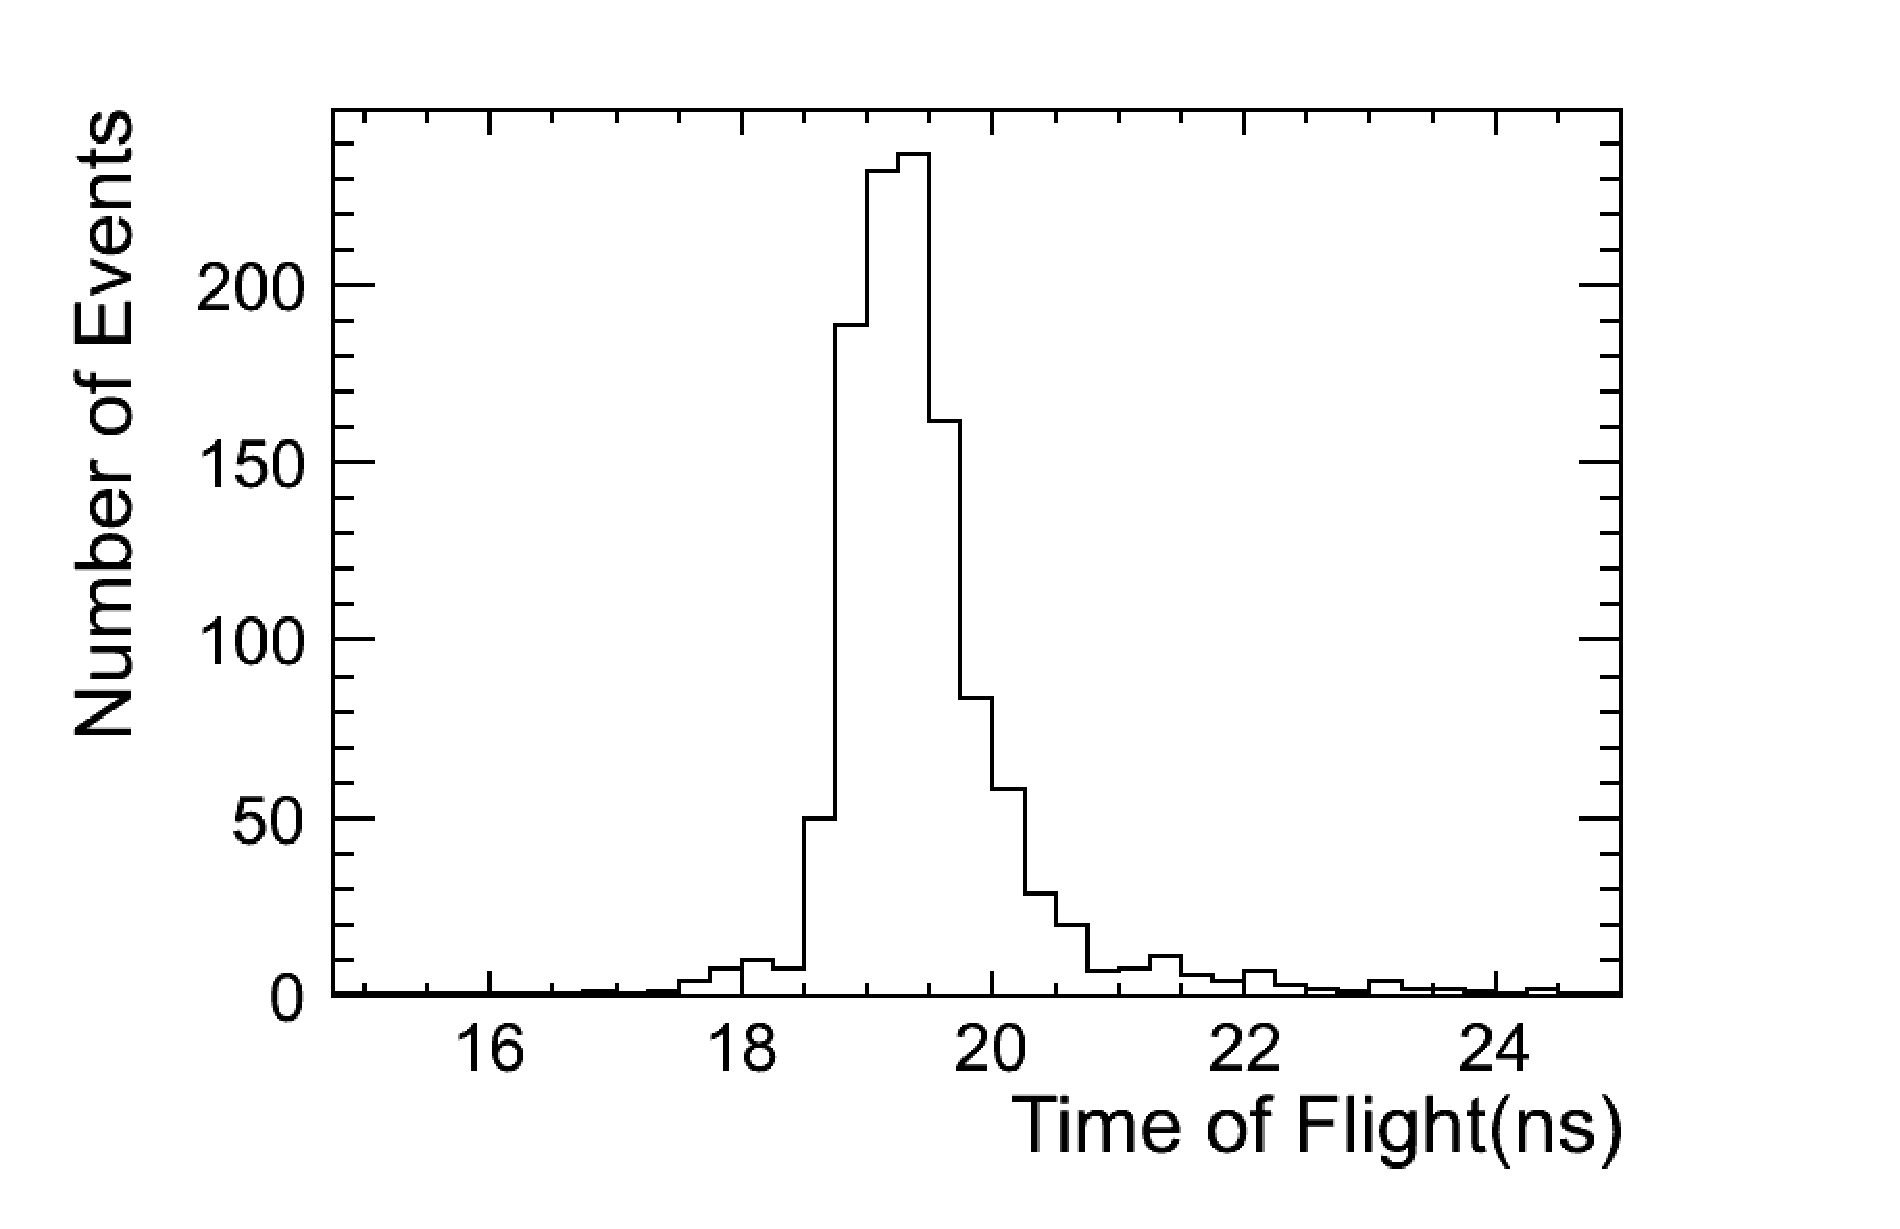
\includegraphics[width=6cm,clip]{fig/TOF_proton.eps}
         \caption{$\rm {\Delta TOF}$ distribution of TOF counters with proton data}
         \label{fig:Proton_tof}
       \end{minipage}
       \begin{minipage}{0.5\hsize}
         \centering
         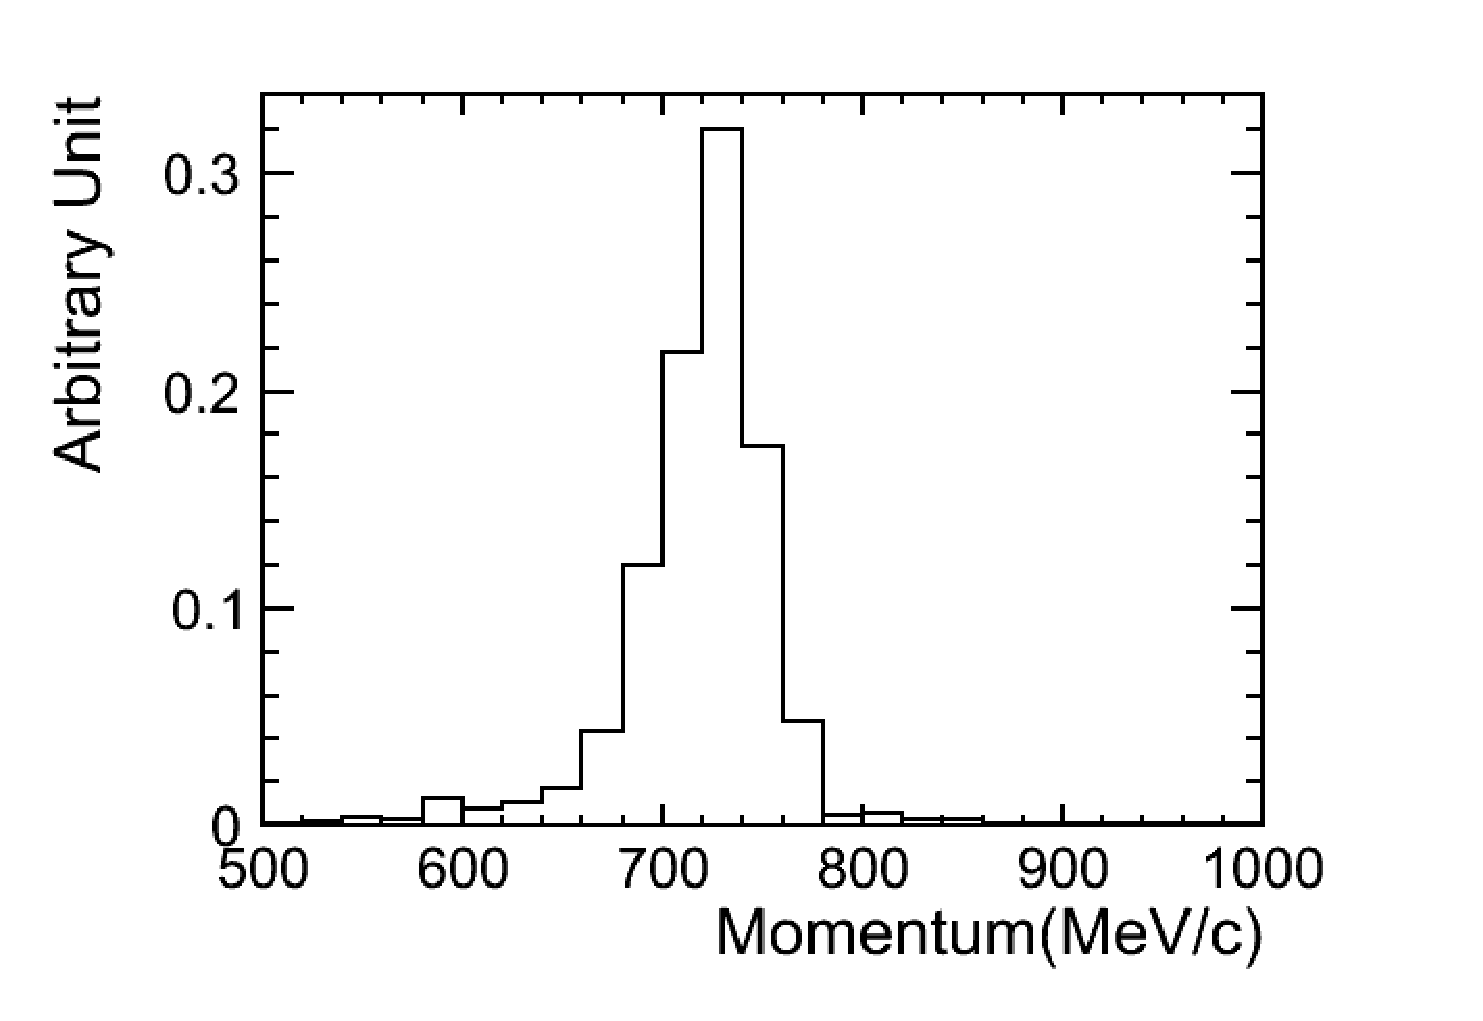
\includegraphics[width=6cm,clip]{fig/Momentum_proton.eps}
         \caption{proton momentum estimated by $\rm {\Delta TOF}$ of TOF counters information}
         \label{fig:Proton_momentum}
       \end{minipage}
     \end{tabular}
   \end{figure} 
   
   \subsection{Beam Position}
   We measured beam profile in front of 250LAr TPC beam window by using plastic scintillation counters.
   Figure \ref{beamprofile_250L} shows beam profile result.
   
   
   \begin{figure}[!htb]
  \centering
  \centering
  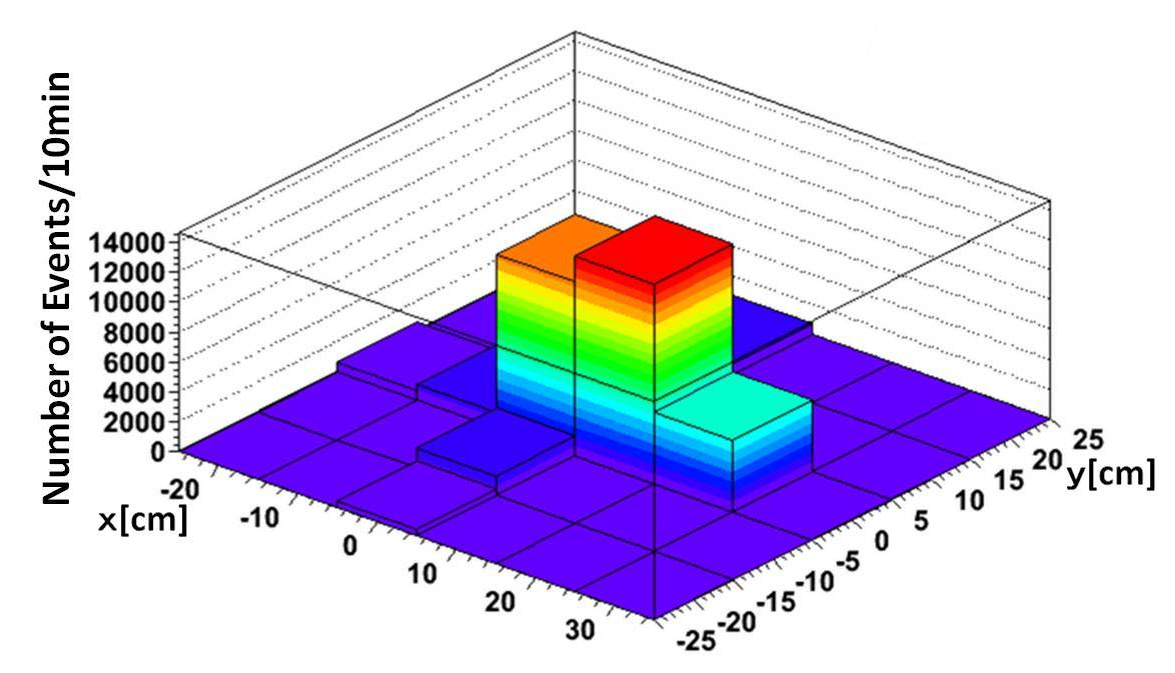
\includegraphics[width=11cm,clip]{./fig/BeamProfile3.eps}
  \caption{Beam profile on the front of 250LAr TPC}
  \label{beamprofile_250L}
\end{figure}

